% siminos/reversal/LC21FT.tex      pdflatex LC21; bibtex LC21
% temporary: siminos/chapter/LC21FT.tex  pdflatex blogCats; biber blogCats
% $Author: predrag $ $Date: 2021-12-24 01:25:20 -0500 (Fri, 24 Dec 2021) $

\section{Deterministic lattice field theory}
\label{s:LC21FT}
%\label{sect:lattDisc}

\renewcommand{\Ssym}[1]{{\ensuremath{m_{#1}}}}
\renewcommand{\source}{\Mm}

%%%%%%%%%%%%%%%%%%%%%%%%%%%%%%%%%%%%%%%%%%%%%%%%%%%%%
% PC 2021-09-26: always harmonize with 1dLatStatC_5_1.svg
\begin{figure}
  \centering
%{(a)}
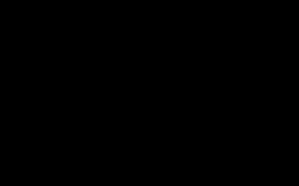
\includegraphics[width=0.50\textwidth]{LC21FieldConfig}
  \caption{\label{LC21FieldConfig}
(Color online)~~~
Discretization of a 1\dmn\ field theory.
Horizontal: $\zeit$ coordinate, with lattice sites marked by dots and
labelled by $\zeit\in\integers$.
(a)
A periodic field $\ssp(\zeit)$, plotted as a function of continuous
coordinate $\zeit$.
(b)
A corresponding discretized period-$5$ {\lattstate}
$\Xx=\cycle{\ssp_0 \ssp_1 \ssp_2 \ssp_3 \ssp_4}$,
with discretized field $\ssp_\zeit$ plotted as a bar
centred at lattice site $\zeit$.
In what follows we use `lattice units' \(a=1\).
          }
\end{figure}
%%%%%%%%%%%%%%%%%%%%%%%%%%%%%%%%%%%%%%%%%%%%%%%%%%%%%

A scalar field $\ssp(x)$ over $d$ Euclidean coordinates can be
discretized by
replacing the continuous space by a $d$\dmn\ hypercubic {integer lattice}
$\lattice$, with lattice spacing $a$, and
evaluating the {field} only on the
lattice points\rf{MonMun94,MunWal00}
\beq
\ssp_z
=
\ssp(x)
    \,,\qquad \qquad x = az= \mbox{lattice point}
    \,,\quad z \in \integers^d
\,,
\ee{LattField}
see \reffig{LC21FieldConfig}.
A given {\em field configuration} (here in one {\spt} dimension)
\beq
\Xx =
\cdots {\ssp}_{-3} {\ssp}_{-2}\,{\ssp}_{-1}\,
       {\ssp}_0\,
      {\ssp}_{1} {\ssp}_{2} {\ssp}_{3} {\ssp}_{4}  \cdots
\,,
\ee{stateSp}
taking any value in system's $\infty$\dmn\ \emph{\statesp}
$\ssp_{z}\in\reals$, occurs with probability
\beq
p(\Xx)\,=\, \frac{1}{Z}\,\e^{-\action[\Xx]}
\,,\qquad Z=Z[0]
\,.
\label{ProbConf}
\eeq
Here $Z$ is a normalization factor, given by the \emph{partition
function}, the integral over probabilities of all
configurations,
\beq
Z[\source]	% = e^{W[\source]}
    \,=\, \int d\Xx\,e^{-\action[\Xx] + \Xx \cdot \source}
    \,,\qquad
d\Xx = \prod_{z}^{\lattice} d\ssp_z
\,,
\ee{partFunct}
where $\source=\{\Ssym{z}\}$ is an external `source' that one can vary
at will, site-by-site, and $\action[\Xx]$ is the action that defines the
theory. %\rf{FieldThe}
The dimension of the partition function integral is the number of lattice
sites $N_\lattice$.
%, \ie, the lattice volume.   % =\Det\lattice$.

Motivated by WKB `semi-classical' or saddle-point
approximations\rf{gutbook} to the partition function \refeq{partFunct},
in this paper we describe their deterministic underpinning, the corresponding
\emph{deterministic} field theory, with partition function built from
solutions to the variational saddle-point condition
\beq
F[\Xx_c]_z =
- \action[\Xx_c]_z + \Ssym{z} =0
\,,\qquad
\action[\Xx]_z=\frac{\delta{\action[\Xx]}}{\delta\ssp_z~}
\,,
\ee{LC21eqMotion}
with a global deterministic solution $\Xx_c$ satisfying this local extremal
condition on every lattice site.
In order to distinguish a \emph{solution} to the Euler–Lagrange equations
\refeq{LC21eqMotion} from an {arbitrary} \emph{field configuration}
\refeq{stateSp}, we refer to the solutions as
\emph{{\lattstate}s}, each a set of lattice site field values
\beq
\Xx_c = \{\ssp_z\}
\,,
\label{1dLattStat}
\eeq
that satisfies the local {condition} \refeq{LC21eqMotion} globally,
over all lattice sites.
For a finite lattice segment $\Xx$, one needs to specify the boundary
conditions ({\bcs}).
%  for the Green's function \refeq{tempCatGreen}.
The companion article \refref{GHJSC16} tackles the Dirichlet {\bcs}, a
difficult, time-translation symmetry breaking, and from the \po\ theory
perspective, a wholly unnecessary, self-inflicted pain. All that one
needs to solve the {\templatt} are the $\period{}$-periodic,
time-translation enforced {\bcs} that we shall use here.
    \PC{2020-02-08}{
Complain about that stupidity clearly both in the intro and in conclusions.
    }
An example is the 1 {\spt} dimension \brick\ of fields of period
$\cl{}=5$ sketched in \reffig{LC21FieldConfig}\,(b),
\beq
\Xx_c = \cycle{\ssp_0 \ssp_1 \ssp_2 \ssp_3 \cdots \ssp_{\cl{}-1}}
\,,
\ee{1dLattStatC_n}
with its infinite repetition --for a sketch, see
\reffig{fig:1dLatStatC_5}\,(1)-- denoted by an overbar.
The first field value $\ssp_0$ in the \brick\ is evaluated on the lattice site 0,
the second $\ssp_1$ on the lattice site 1,
the $\cl{}$th $\ssp_{\cl{}}=\ssp_0$ on the lattice site $\cl{}$,
with $k$th lattice site field value $\ssp_{k}=\ssp_{\ell}$,
where $\ell=k$~(mod$\cl{}$).

What we call here a chaotic `field' at a discretized spacetime lattice
site $z$, a solid state physicist would call the state of a `particle' at
crystal site $z$, coupled to its nearest neighbors. A solid state
physicist endeavours to understand $N$-particle chaotic systems in
many-body or `large $N$' settings, where in practice any $N$ larger than 2
is `large'. Chaotic field theory is {\em ab initio} formulated for infinite
time and infinite space lattice, but its periodic theory description is
-thanks to hyperbolicity-- computationally powerful already for $N=2, 3,
\cdots$, where $N$ is the number of sites in Bravais cells that tile the
spacetime.

Each {\lattstate} is a distinct deterministic solution $\Xx_c$ to the
discretized Euler–Lagrange equations \refeq{LC21eqMotion}, so its
probability is a $N_\lattice$\dmn\ Dirac delta function
(that's what we mean by the system being \emph{deterministic})
\beq
p_c(\Xx)\,=\, \frac{1}{Z}\,\delta(F[\Xx_c-\Xx])
\,.
\label{DiracDeltaExp}
\eeq

% To comfort sceptics, we verify
In \refsect{s:LC21notHill} we  verify that this
definition agrees with the customary for\-ward-in-time \FP\ probability
evolution\rf{CBmeasure} (see \toChaosBook{section.19.2}{sect.~19.2}). The
new, field-theoretical formulation is vastly preferable to the
for\-ward-in-time formulation when it comes to higher \spt\
dimensions\rf{CL18}.

As is case for a WKB approximation\rf{gutbook}, the {deterministic} field
theory partition sum has support only on lattice field values that are
solutions to the variational saddle-point condition \refeq{LC21eqMotion},
and the partition function \refeq{ProbConf} is now a sum over
configuration \statesp\ \refeq{stateSp} \emph{points},
\bea
Z_c[\source] &=& \sum_c e^{N_\lattice W_c[\source]}
            \continue
e^{N_\lattice W_c[\source]}
    &=& \int_{\pS_c} d\Xx\,\delta(F[\Xx])
    \,=\, \frac{1}{\left|\Det\jMorb_c\right|}
\,,
\label{ClassPartitF}
\eea
where $\pS_c$ is a small neighborhood of  $\Xx_c$, and we refer to
the $[N_c\!\times\!N_c]$ matrix of second derivatives
\beq
(\jMorb_c)_{z'z} = \frac{\delta F[\Xx_c]_{z'}}{\delta \ssp_{z}}
             = \action[\Xx_c]_{z'z}
\ee{jacobianOrb}
as the \emph{\jacobianOrb}.

In what follows, we shall almost exclusively deal only with deterministic field
theory and omit the subscript `$c$' in $\Xx_c$ througout.

\subsection{Lattice Laplacian}
\label{s:LC21lattLap}


Let's have a look at the lattice free field theory action
\beq
\action_0[\Xx]=
          \frac{1}{2}\transp{\Xx}\left(-\Box + {\mu}^2\mathsf{1} \right)\Xx
\,,
\ee{LC21freeAction}
where the `discrete Laplace operator', `central difference operator', or
the `graph Laplacian'%
\rf{PerViv,Pollicott01,Cimasoni12,MraRin12,GodRoy13,Pozrikidis14}
\beq
\Box\,\ssp_z =
    % \frac{1}{2d}
    \sum_{||z'-z||=1} \!\! (\ssp_{z'} - \ssp_z)
 \quad \mbox{for all} \ z,z' \in \lattice % \integers^d
% \,,\quad ||i||:=\sum_{k=1}^{d}|i_k|
% \,,
\ee{LC21:Lap}
is the average of the lattice field variation $\ssp_{z'}-\ssp_z$
over the sites nearest to the site $z$.
For example, for a hypercubic lattice in one and two dimensions this
discretized Laplacian is given by
\bea
\Box\,\ssp_\zeit &=& \ssp_{\zeit+1} - 2\,\ssp_{\zeit} + \ssp_{\zeit-1}
    \label{LC21LaplTime}\\
\Box\,\ssp_{j\zeit}
     &=&
\ssp_{j,\zeit+1} + \ssp_{j+1,\zeit} - 4\,\ssp_{j\zeit}
                 + \ssp_{j,\zeit-1} + \ssp_{j-1, \zeit}
\,.
\label{LC21LaplSpaceTime}
\eea

For action \refeq{LC21freeAction} this is the discretized
{\sPe}\rf{FetWal03}, also known as the {Yukawa} or Klein–Gordon
equation, where  ${\mu}^2>0$ is the Klein–\-Gordon mass-squared.
An example is the Gutkin and Osipov\rf{GutOsi15} \catlatt\ in  $d=2$
dimensions\rf{CL18}, an Arnold cat map-inspired scalar field theory  of
form \refeq{LC21freeAction} for which the Euler–\-Lagrange
equation \refeq{LC21eqMotion} is a 5-term recurrence relation
\beq
      -\ssp_{j,\zeit+1} - \ssp_{j,\zeit-1}
+ 2{s}\,\ssp_{j\zeit}
     - \ssp_{j+1,\zeit} - \ssp_{j-1, \zeit}
     =  \Ssym{j\zeit}
\,,
\ee{CatMap2d}
where we refer to parameter ${s}$, related to the Klein-Gordon mass in
\refeq{LC21freeAction} by ${\mu}^2=d({s}-2)$, as the `stretching
parameter'.

\subsection{1\dmn\ lattice field theories}
\label{s:LC21FT1d}

Discrete time evolution is frequently recast into a 1\dmn\ temporal
lattice field theory form, essentially by anyone who rewrites a
dynamical systems discrete time evolution problem as a $k$-point recurrence,
for example in
\refrefs{FeHa82,noisy_Fred,conjug_Fred,diag_Fred}.
As already in one \spt\ dimension there is much to be learned about the
role symmetries play in solving lattice field theories, that is what we
will focus on in this paper (time-reversal
\refsects{s:latt1d}{sect:LC21Lind1d}), with the $2$\dmn\ \spt\ field
theories discussed in the sequel\rf{CL18}.

We shall consider scalar field theories of polynomial type, with a local
potential%
\rf{FriMil89,DulMei00,LiMal04,AnBoBa17,AnBoBa18,Anastassiou21}
\beq
V(\ssp_\zeit) = \frac{g}{k}\ssp_{\zeit}^k - \Ssym{\zeit}\ssp_{\zeit}
\ee{polynPotent}
on each  1\dmn\ lattice site $\zeit$ added to the free field theory
action \refeq{LC21freeAction}. The discrete Euler–Lagrange equations
\refeq{LC21eqMotion} now take form of 3-term recurrence, second-order
difference equations
\bea
- \ssp_{\zeit+1} + V'(\ssp_{\zeit}) - \ssp_{\zeit-1}
    &=&
0  % was \Ssym{\zeit}
\,.  %\qquad  \ssp_{\zeit} \in [0,1)
\label{LC21:1dTempFT}% \refeq{LC21:1dTempFT}
\eea

We start with the first order difference equation that we call
`{temporal Bernoulli}' (\refsect{s:coinToss}),
\bea
- \ssp_{\zeit+1} + {s}\,\ssp_{\zeit}
    \qquad\quad\;
    &=&
\Ssym{\zeit}
%\,,\qquad  \ssp_{\zeit} \in [0,1)\,,
\label{LC21:1dBernLatt}    % labelled {1stepDiffEq} elsewhere
\eea
in order to motivate the second-order difference
Euler–Lagrange equations \refeq{LC21:1dTempFT}
that we call, in the cases considered here,
the `{\templatt}' (\refsect{s:kickRot}),
`{\henlatt}' (\refsect{s:henlatt}), and
`temporal {$\phi^4$} theory'  (\refsect{s:phi4latt}), respectively:
\bea
- \ssp_{\zeit+1}  +  \,{s}\,\ssp_{\zeit} - \ssp_{\zeit-1}
    &=&
\Ssym{\zeit}
%\,,\qquad  \ssp_{\zeit} \in [0,1)
\label{LC21:1dTemplatt}\\
- \ssp_{\zeit+1} + {a}\,\ssp_{\zeit}^2 - \ssp_{\zeit-1}
    &=&
\Ssym{\zeit}
%\,,\qquad  \Ssym{\zeit}=2
\label{LC21:1dHenlatt}\\
- \ssp_{\zeit+1} + {g}\,\ssp_{\zeit}^3 - \ssp_{\zeit-1}
    &=&
\Ssym{\zeit}
%\,.
\label{LC21:1dPhi4}
\eea
Qualifier `temporal' is used here to emphasize that we view 1\dmn\
examples as special cases of `\spt' field theories; much of our
methodology for $d$\dmn\ deterministic field theories can be profitably
explained by working out $1$\dmn\ field theories.
Lurking here is the totality of the map-iteration dynamical systems
theory, but the reader will find it more profitable, and less confusing,
to think of these simply as lattice problems, and forget that the index
$\zeit$ often stands for `time'.

So, what is a `chaotic', or `turbulent' field theory?
As we shall see, all of the above, as well as their
higher\dmn\ \spt\ siblings are `chaotic' for sufficiently strong `stretching
parameters' or `coupling constants'  ${s}$, ${a}$ or ${g}$.
Our goal here is to make this `{\spt} chaos' tangible and precise, by
acquainting the reader what we believe are
some of the simplest, most elegant examples chaotic field theories.
